\documentclass{scalatekids-article}
\usepackage[official]{eurosym}
\usepackage[english]{babel}
\begin{document}
\lfoot{Developer Manual 1.0.0}
\newgeometry{top=3.5cm}
\begin{titlepage}
  \begin{center}
    \begin{center}
      
\includegraphics[width=10cm]{sklogo.png}
    \end{center}
    \vspace{1cm}
    \begin{Huge}
      \begin{center}
        \textbf{Developer Manual}
      \end{center}
    \end{Huge}
    \vspace{11pt}
    \bgroup
    \def\arraystretch{1.3}
    \begin{tabular}{r|l}
      \multicolumn{2}{c}{\textbf{Document Information}} \\
      \hline
      \setbox0=\hbox{0.0.1\unskip}\ifdim\wd0=0pt
      \\
      \else
      \textbf{Version} & 1.0.0\\
      \fi
      \textbf{Editing} & \multiLineCell[t]{\\}\\
      \textbf{Verification} & \multiLineCell[t]{\\}\\
      \textbf{Approvation} & \multiLineCell[t]{}\\
      \textbf{Use} & External\\
      \textbf{Distribution List} & \multiLineCell[t]{ScalateKids\\Prof. Tullio Vardanega\\Prof. Riccardo Cardin}\\
    \end{tabular}
    \egroup
    \vspace{22pt}
  \end{center}
\end{titlepage}
\restoregeometry
\clearpage
\pagenumbering{Roman}
\setcounter{page}{1}
\begin{flushleft}
  \vspace{0cm}
  {\large\bfseries History log}
\end{flushleft}
\vspace{0cm}
\begin{center}
  \begin{longtable}{| l | l | l | l | p{5cm} |}
    \hline
    Version & Author & Role & Date & Description \\
    \hline
    1.0.0 & Michael Munaro & Project Manager & 2016-05-15 & Document approved\\
    \hline
    0.11.0 & & & 2016-05-15 & Verified subsection 2.1.1 - Server-side general structure\\
    \hline
    0.10.1 & & Programmer & 2016-05-15 & Improvements to section 2.1 - Installation, added subsection 2.1.1 - Server-side general structure\\
    \hline
    0.10.0 & & & 2016-05-15 & Verified section 2.3.0.5 - Contribute and relative subsections\\
    \hline
    0.9.0 & & & 2016-05-15 & Verified improvements in section 2.1.1\ -\ Building from sources, build configuration for CLI and Server\\
    \hline
    0.8.3 & & Programmer & 2016-05-15 & Added section 2.3.0.5 - Contribute and relative subsections \\
    \hline
    0.8.2 & & Programmer & 2016-05-15 & Improved section 2.1.1\ -\ Building from sources, added build configuration for CLI\\
    \hline
    0.8.1 & & Programmer & 2016-05-14 & Improved section 2.1.1\ -\ Building from sources, added build configuration for server\\
    \hline
    0.8.0 & & & 2016-05-14 & Verified sample configuration in section 2.1\ -\ Installation\\
    \hline
    0.7.1 & & Programmer & 2016-05-14 & Improved section 2.1\ -\ Installation, added sample configuration\\
    \hline
    0.7.0 & & & 2016-05-13 & Verified section 2.1.1\ -\ Building from sources\\
    \hline
    0.6.1 & & Programmer & 2016-05-13 & Added section 2.1.1\ -\ Building from sources\\
    \hline
    0.6.0 & & & 2016-05-13 & Verified section 2.1\ -\ Installation\\
    \hline
    0.5.1 & & Programmer & 2016-05-13 & Added section 2.1\ -\ Installation\\
    \hline
    0.5.0 & & & 2016-05-13 & Verified section 2.1.1\ -\ Building from sources\\
    \hline
    0.4.1 & & Programmer & 2016-05-13 & Added section 2.1.1\ -\ Building from sources\\
    \hline
    0.4.0 & & & 2016-05-13 & Verified section 2.4.0.4\ -\ Failure management\\
    \hline
    0.3.0 & & & 2016-05-13 & Verified sections 2.4.0.2\ -\ Profile management, 2.4.0.3\ -\ Collections operations and relative subsections\\
    \hline
    0.2.2 & & Programmer & 2016-05-13 & Added section 2.4.0.4\ -\ Failure management\\
    \hline
    0.2.1 & Andrea Giacomo Baldan & Programmer & 2016-05-13 & Added sections 2.4.0.2\ -\ Profile management, 2.4.0.3 - Collections operations and relative subsections\\
    \hline
    0.2.0 &  &  & 2016-05-12 & Verified section 2.3.1\ -\ Quick start, 2.4\ -\ More in depth: common operations and 2.4.1 - Authentication\\
    \hline
    0.1.2 & Andrea Giacomo Baldan & Programmer & 2016-05-12 & Added section 2.4\ -\ More in depth: common operations and 2.4.1 - Authentication\\
    \hline
    0.1.1 & Andrea Giacomo Baldan & Programmer & 2016-05-12 & Added section 2.3.1\ -\ Quick start\\
    \hline
    0.1.0 &  &  & 2016-05-10 & Verified section 2: Actorbase Usage and subsection 2.3\\
    \hline
    0.0.2 & Andrea Giacomo Baldan & Programmer & 2016-05-10 & Added section 2: Actorbase Usage and subsection 2.3\\
    \hline
    0.0.1 & Andrea Giacomo Baldan & Programmer & 2016-05-10 & Created document structure\\
    \hline
  \end{longtable}
\end{center}
\tableofcontents
\newpage
\pagenumbering{arabic}
\section{Summary}

\subsection{Document purpose}

This document aims to describe the procedures and methods to use in order to take
advantage of \textbf{Actorbase} features, including installation steps and configuration
available to users.

\subsection{Product purpose}

The purpose of the project is the realization of a key-value type
NoSQL\footnote{\label{nosql}} database, massively concurrent and oriented to the
management of heavy load of data by using the actor\footnote{A computational entity
that, in response to a message it receives, can send messages to other actors,
create new ones, change its behaviour for the next message incoming\label{actor}}
model.

% \subsection{References}

% \subsubsection{Normative} % TODO check, translated with wordreference

% \subsubsection{Informational} % TODO check, translated with wordreference

% TODO parte server: installazione, configurazione, accensione, spegnimento

% TODO mettere una sezione in cui si spiega cosa è una collection, un item, tutto quel che bisogna descrivere

% TODO bisogna spiegare come devnoon essere formati i file pel l'import

%%%%%%%%%%%%%%%%%%%%%%%%%%%%%%%%%%%%%%%%%%%%%%%%%%%%%%%%%%%%%%%%%%%%
%%% INSTALLATION PART                    %%%
%%%%%%%%%%%%%%%%%%%%%%%%%%%%%%%%%%%%%%%%%%%%%%%%%%%%%%%%%%%%%%%%%%%%


%%%%%%%%%%%%%%%%%%%%%%%%%%%%%%%%%%%%%%%%%%%%%%%%%%%%%%%%%%%%%%%%%%%%
%%%%%%%%%%%% MACHETE                   %%%%%%%%%%%%
%%%%%%%%%%%%%%%%%%%%%%%%%%%%%%%%%%%%%%%%%%%%%%%%%%%%%%%%%%%%%%%%%%%%


\section{Actorbase usage}

\subsection{Installation}

\subsubsection{Minimum requirements}

In addition to JVM version 8, for a pleasing experience \textbf{Actorbase} requires at minimum:
\begin{itemize}
\item RAM:\@1 GB;\@
\item Disk space: 512MB;\@
\item CPU: x64 - 1.2GHz;
\end{itemize}

\subsubsection{Installation steps}

The system is basically constituted of two JAR (Java Archive) shipped with all
dependencies libraries, there are just a few steps to follow to have the system
running and ready to receive commands:
\begin{itemize}
\item run \verb=actorbase.jar= in a shell\footnote{A command-line interpreter\label{shell}};
\item run \verb=actorbasecli.jar= in a second shell\textsuperscript{\ref{shell}}.
\end{itemize}
That's really all for a basic usage, and the procedure is the same for
\textit{Windows} 10, \textit{Ubuntu 14.04 LTS}, \textit{OSX - El
  Capitan} and following versions, though it's possible to give \textbf{Actorbase} a custom configuration by
running:

 \begin{figure}[H]
   \begin{center}
     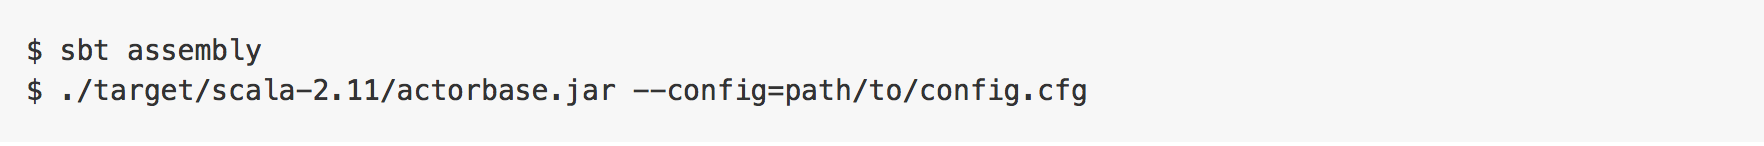
\includegraphics[width=0.9\textwidth,keepaspectratio]{RQ/DevManual/Actorbase-BuildBin.png}
     \caption{Actorbase: build binaries with custom configuration}
   \end{center}
 \end{figure}

\textbf{Configuration sample}

 \begin{figure}[H]
   \begin{center}
     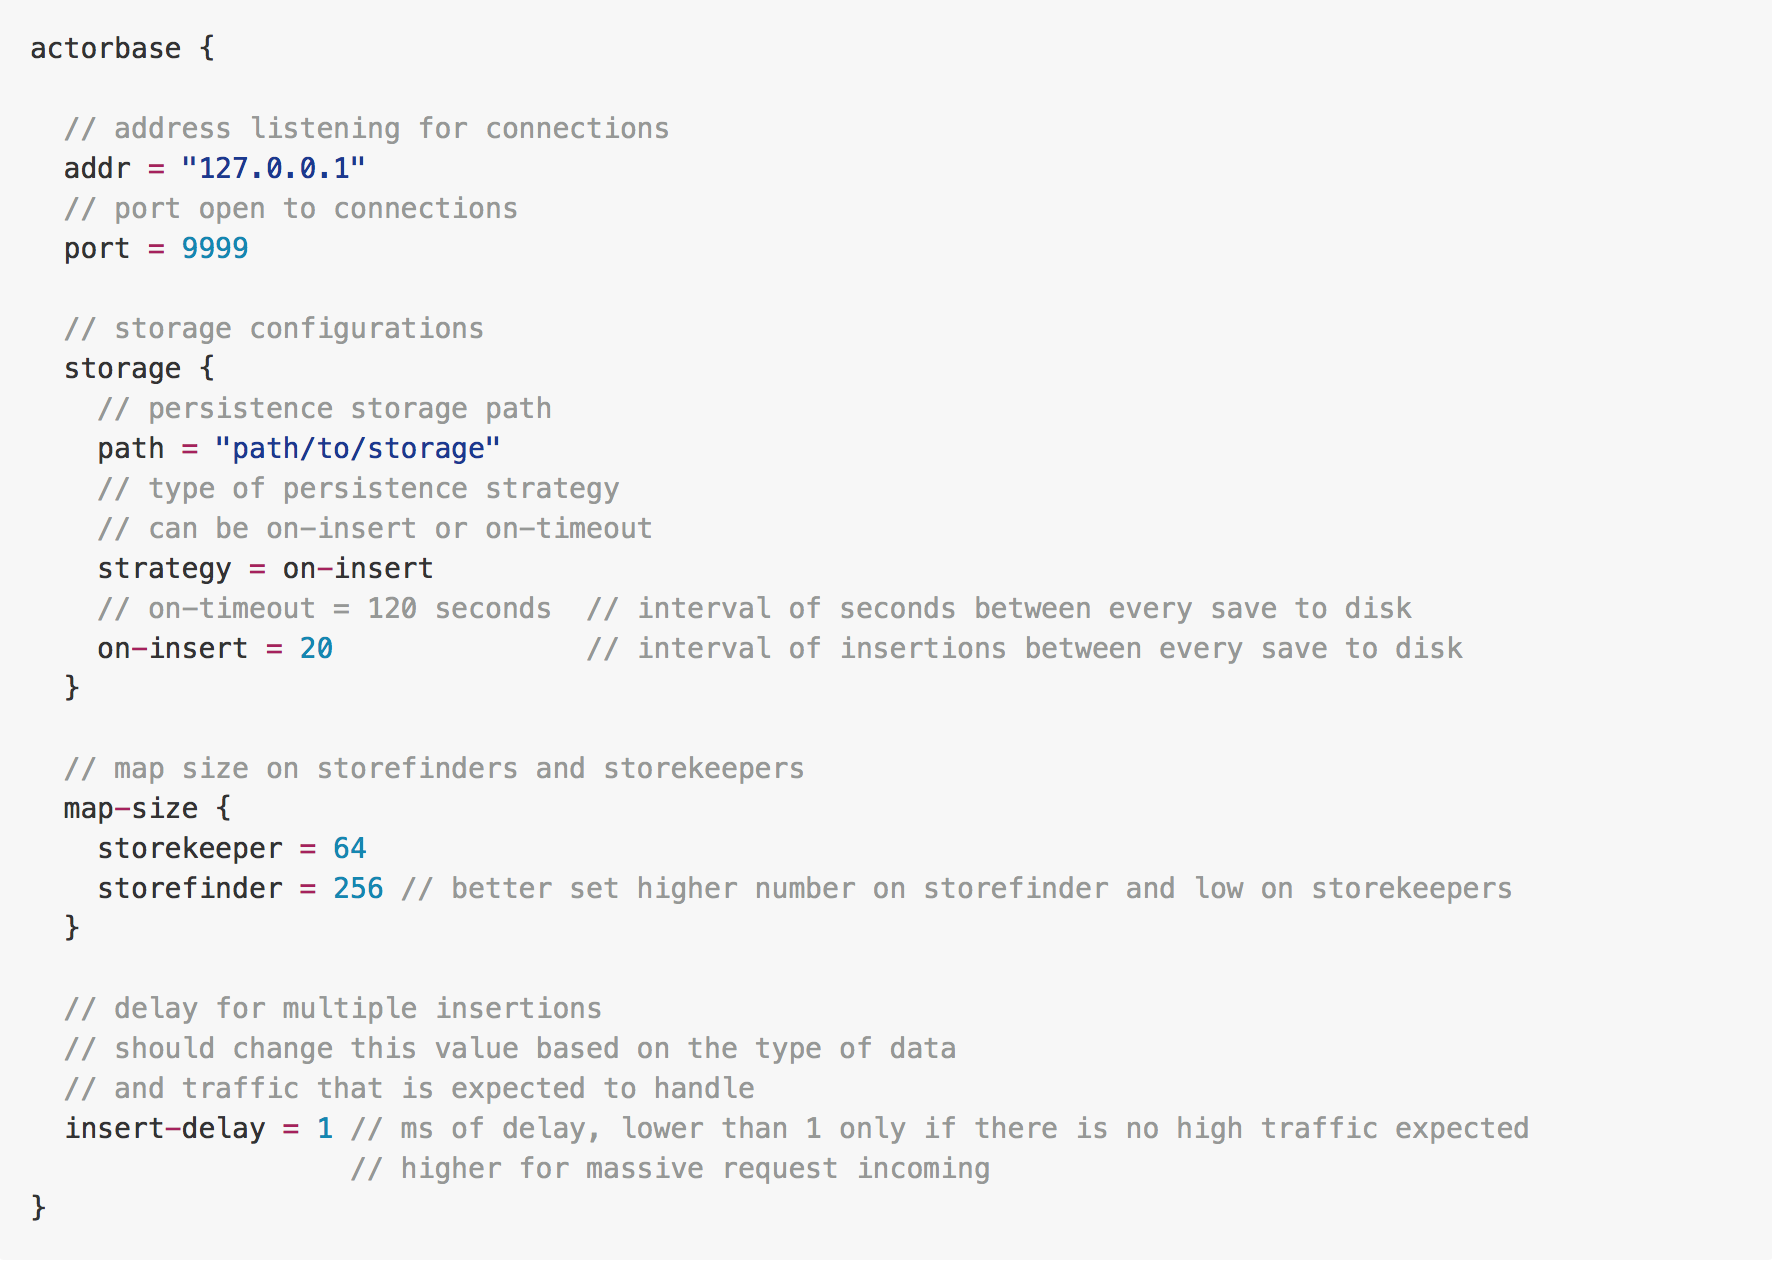
\includegraphics[width=0.9\textwidth,keepaspectratio]{RQ/DevManual/Actorbase-Config.png}
     \caption{Actorbase: configuration sample}
   \end{center}
 \end{figure}

The \textit{--config=path/to/config.cfg} is optional.

As shown in the image, there is a part of the configuration dedicated to the
distribution of the load between multiple nodes in a cluster\footnote{A set of
loosely or tightly connected computers that work together, so that they can be
viewed as a single system\label{cluster}}, \textbf{Actobase} is in fact a
scale-out\footnote{Method of adding more resources by adding more nodes to the
cluster\label{cleout}} oriented system, and it is possible to set all
cluster\textsuperscript{\ref{cluster}} configurations offered by Akka library.

\subsubsection{Server-side general structure}

As previously stated, \textbf{Actorbase} is an application conceived to be used in a distributed fashion,
balancing load between multiple nodes as shown below:

\begin{figure}[H]
  \begin{center}
    \includegraphics[width=0.9\textwidth,keepaspectratio]{RQ/DevManual/ClusterP.png}
    \caption{Actorbase: load-balancing general view}
  \end{center}
\end{figure}

For every incoming connection a dedicated actor\textsuperscript{\ref{actor}}, named clientactor\footnote{An actor dedicated
exclusively to handle incoming request from clients connected from outside the
system}, is spawned; it is responsible for all incoming requests from the
client that is connected, and his main role is to forward these requests directy to the
main\footnote{An actor dedicated to the routing of incoming data to subordinated
actors and to the management of the latter\label{main}}
actors\textsuperscript{\ref{actor}} equally distributed across the nodes of a
cluster\textsuperscript{\ref{cluster}}. In this way, with
main\textsuperscript{\ref{main}} actors\textsuperscript{\ref{actor}} breeding
their own hierarchy of subordinates, all incoming data is spread across the
cluster\textsuperscript{\ref{cluster}} network.

\subsubsection{Building from sources}

\textbf{Actorbase} was conceived and developed using SBT (Simple Building Tool) as building and dependencies
manager tool making the compilation and building from sources extremely easy to achieve just by adding a
\verb=build.sbt= file inside a Maven-like folder tree:

\textbf{Server side}

 \begin{figure}[H]
   \begin{center}
     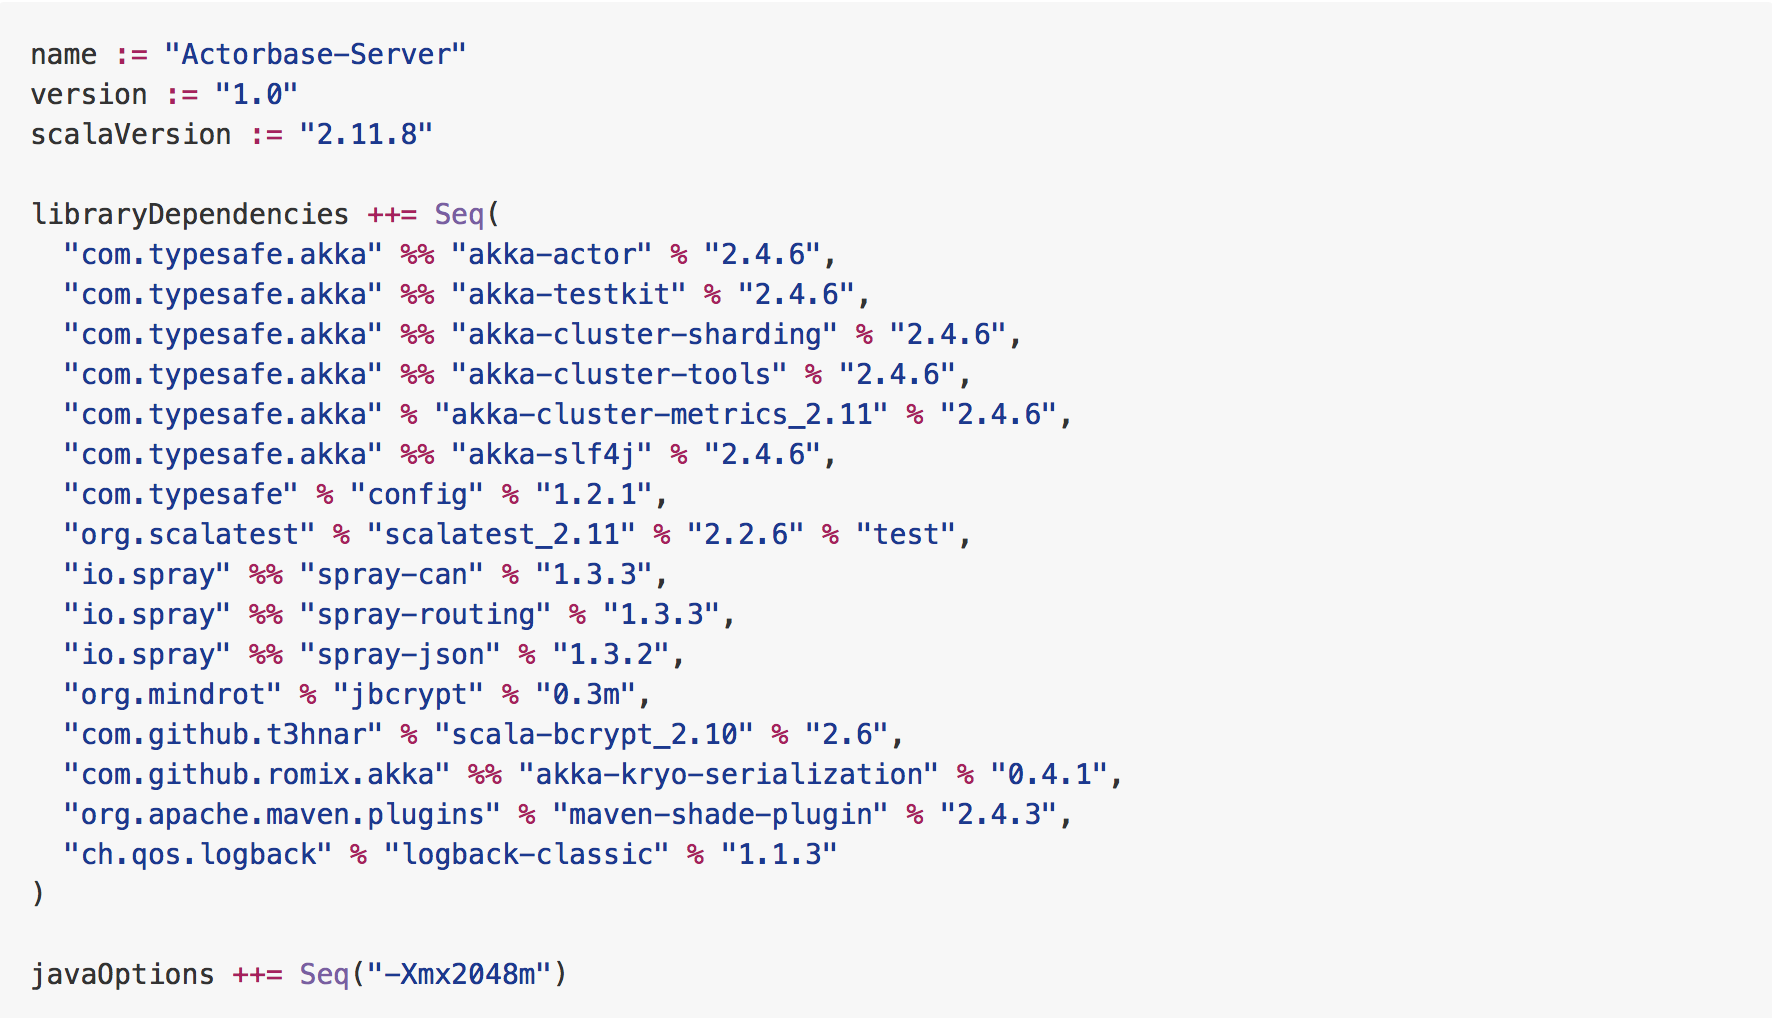
\includegraphics[width=0.9\textwidth,keepaspectratio]{RQ/DevManual/Actorbase-FromSourceSbt.png}
     \caption{Actorbase: build.sbt sample to build from sources}
   \end{center}
 \end{figure}

\textbf{CLI}

 \begin{figure}[H]
   \begin{center}
     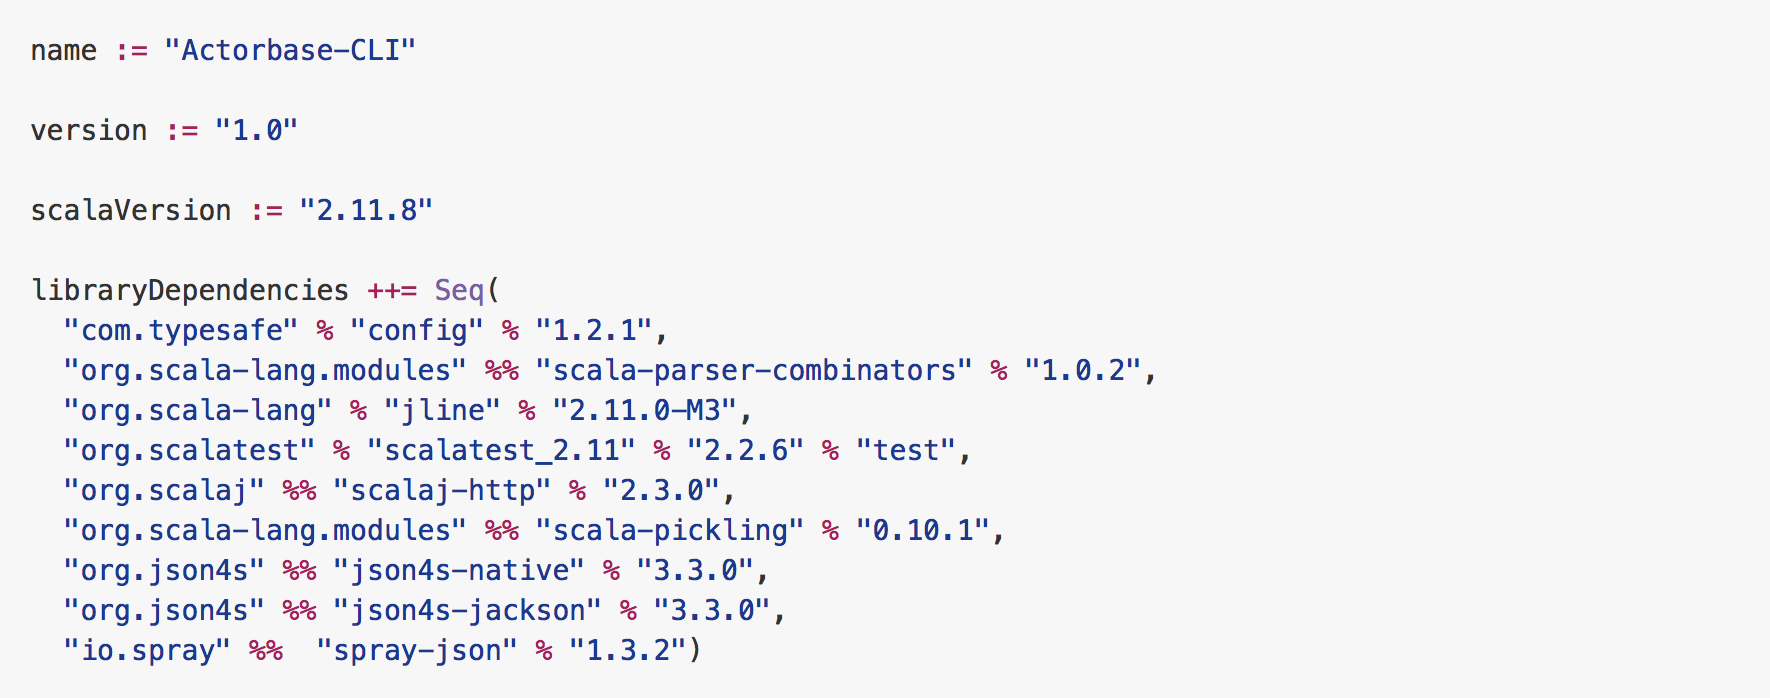
\includegraphics[width=0.9\textwidth,keepaspectratio]{RQ/DevManual/Actorbase-FromSourceSbtCLI.png}
     \caption{Actorbase-CLI: build.sbt sample to build from sources}
   \end{center}
 \end{figure}

As shown in the image, there are some external libraries needed to build the system:
\begin{itemize}
\item \textbf{Spray:} An open source toolkit for building REST/HTTP-based
  integration layers on top of Scala and Akka; mainly used for the server
  component in order to expose communication API and to
  Marshall\footnote{The act of transforming the memory of an object to a data format suitable
    for storage or transmission, e.g.\ serialization} database contents.
\item \textbf{scala-pickling:} An authomatic serialization framework made for
  Scala; mainly used in the driver component in order to serialize and
  deserialize objects in a fast and transparent way;
\item \textbf{scalaj-http:} A fairly simple http library for Scala, used in the
  driver component in order to establish a communication with the REST API server;\
\item \textbf{json4s:} Used in the driver component to expose a pretty formatted
  JSON (JavaScript Object Notation) version of the data retrieved from the server;
\item \textbf{scala-bcrypt:} Scala version of the encryption library Bcrypt,
  used on the server side to store hashes of sensitive data;
\item \textbf{Akka:} A toolkit and runtime environment to build highly concurrent,
  distributed, and resilient message-driven applications on the JVM;\ it is the core of
  the system and it is used in the server-side component.
\end{itemize}

%%%%%%%%%%%%%%%%%%%%%%%%%%%%%%%%%%%%%%%%%%%%%%%%%%%%%%%%%%%%%%%%%%%%
%%% DRIVER PART                          %%%
%%%%%%%%%%%%%%%%%%%%%%%%%%%%%%%%%%%%%%%%%%%%%%%%%%%%%%%%%%%%%%%%%%%%

\subsection{ActorbaseDriver: Using Actorbase from inside a Scala source}

<<<<<<< HEAD
Actorbase is essentially an actor\textsuperscript{\ref{actor}} system built upon a server component that
exposes some API forming a RESTful web service. To facilitate the use from
inside a Scala source, a driver has been developed in order to allow the
usage of all features that \textbf{Actorbase} provides.\\
=======
Actorbase is essentially an actor\textsuperscript{\ref{actor}} system built upon
a server component that exposes some API forming a RESTful web service. To
facilitate the use from inside a Scala source, it has been developed a driver in
order to allow the usage of all features that \textbf{Actorbase} provides.\\
>>>>>>> 285139fa5d3f3a3faefb91c9ae32450b851a64fb

\subsubsection{Quick Start: a generic example}

The most common operations include:
\begin{itemize}
\item Authentication;
\item Profile management operations;
\item Collections operations;
\item Administrative operations.
\end{itemize}

\begin{figure}[H]
  \begin{center}
    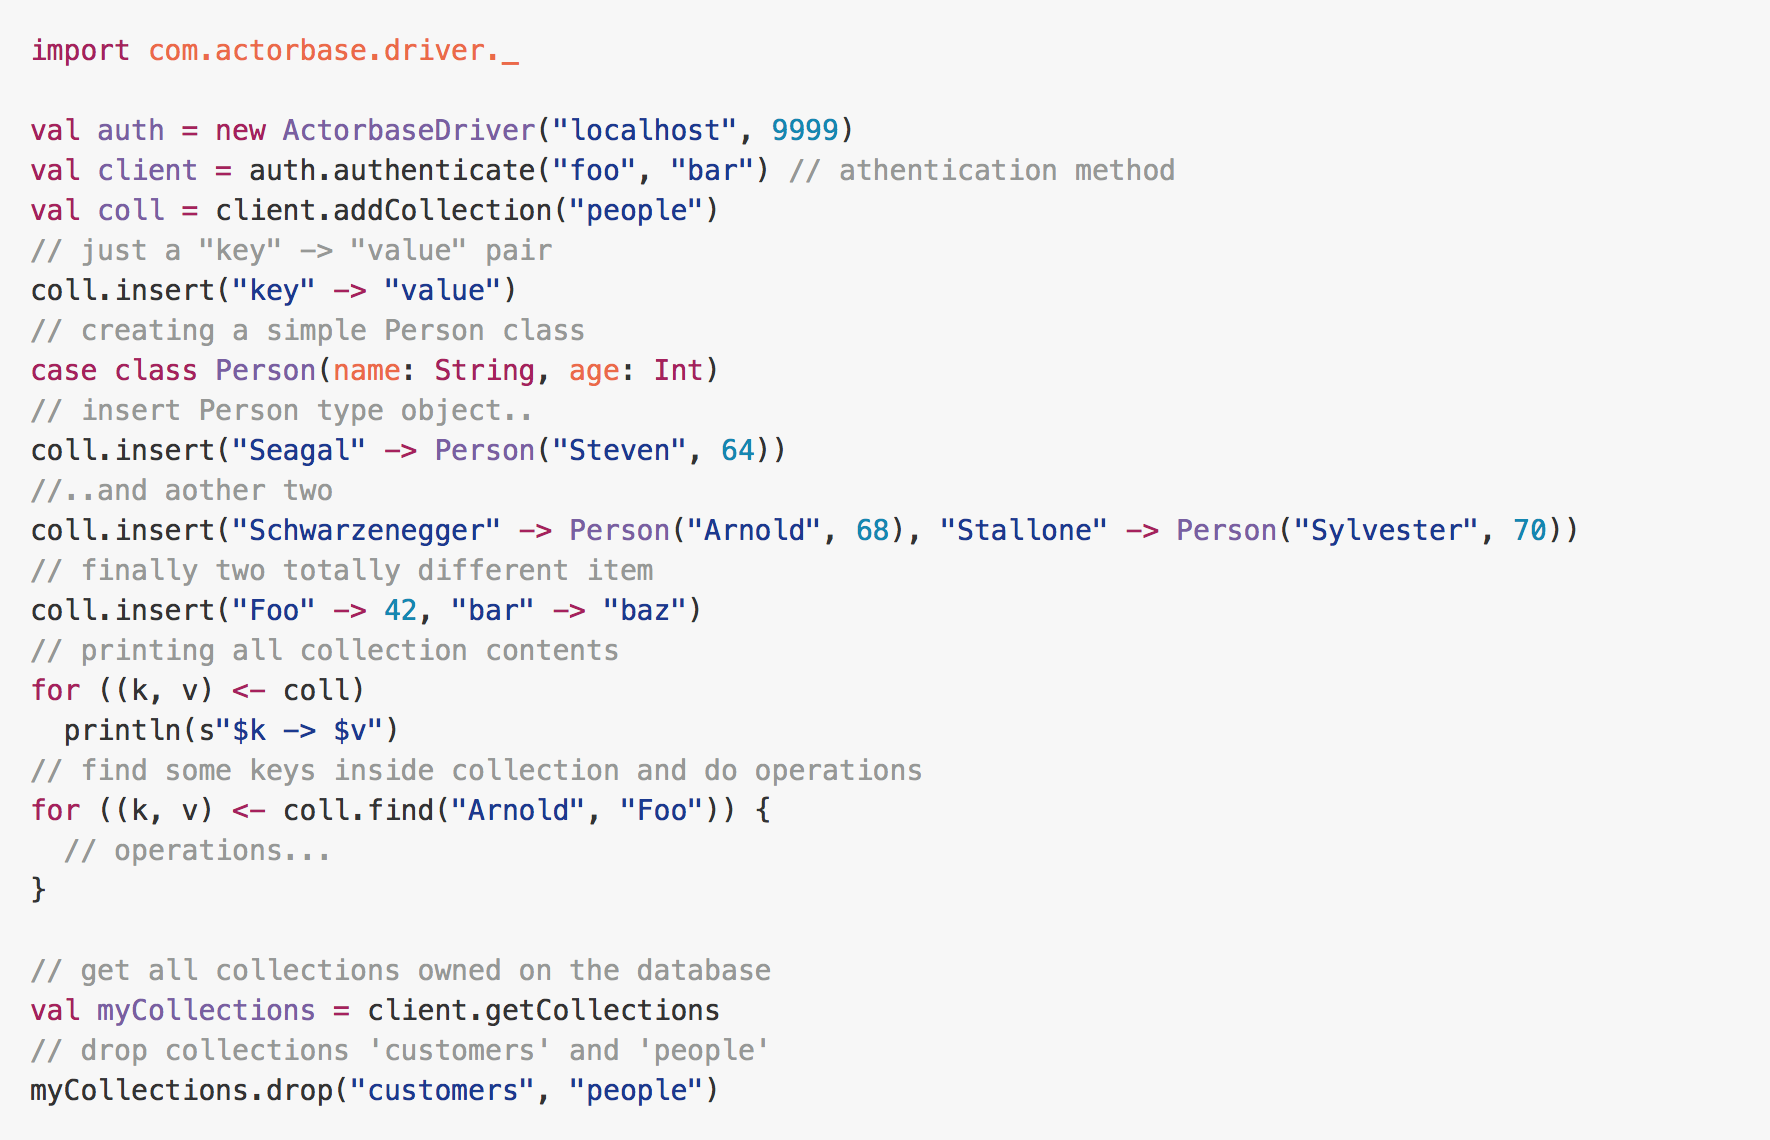
\includegraphics[width=0.9\textwidth,keepaspectratio]{RQ/DevManual/Driver-Common.png}
    \caption{Driver usage: Generic example}
  \end{center}
\end{figure}

These are some of the most common operations that the driver allows the user to do,
there is not too much boilerplate\footnote{A section of code that has to be
  included in many places with little to no alteration.} code, and it is possible
to make operations directly on objects representing \textbf{Actorbase}
collections\footnote{A data-structure constituted by a list of key-value items\label{coll}}
in a purely OOP (Object Oriented Programming) fashion.\\ As explained in
the snippet\footnote{A programming term for a small region of reusable code.}
image these objects also retain some of the common functional constructs (e.g.
foreach), so it's possible to apply custom functions to every item of the
collection.

\subsection{More in depth: common operations}

\paragraph{Authentication}

Although in the future there may be the possibility to make some
operations as an anonymous user, at the current state the only possible action
that a non-logged-in user can do with \verb=ActorbaseDriver= is the authentication.
This method sends a login request to the server-side of the system and, according
to the response, it will return an \verb=ActorbaseService=\footnote{Main class,
  contains all collection management methods\label{ActorbaseServices}} or an
\verb=ActorbaseAdminServices=\footnote{Defined trait, contains some
  administrative functionality as dependency added to
  ActorbaseServices\label{AdminServices}}. These two objects give the methods to
actually make all operations on the database, the main difference is that
\verb=ActorbaseAdminServices=\textsuperscript{\ref{AdminServices}} allows to do
some high-level administrative operations on the users and the
collections\textsuperscript{\ref{coll}} of the system.\\
Authentication method could raise \textbf{WrongCredentialExc} exception, in case
 wrong credentials has been sent to the server.

\paragraph{Profile management}

\textit{ActorbaseDriver} provides a method to modify the current password,
associated to an user profile.
e.g.:
 \begin{figure}[H]
   \begin{center}
     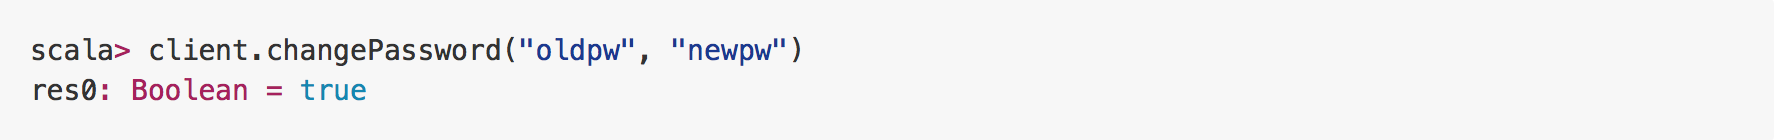
\includegraphics[width=0.9\textwidth,keepaspectratio]{RQ/DevManual/Driver-UserManagement.png}
     \caption{Driver usage: insertion methods}
   \end{center}
 \end{figure}
This method could raise:
\begin{itemize}
\item \textbf{WrongPasswordExc} In case the user made a mistake inserting the current password;
\item \textbf{WrongNewPasswordExc} In case the new password does not meet the \textbf{Actorbase} password rules.
\end{itemize}

\subparagraph{Credential rules}
% TODO: Complete
Usernames can not be an empty string or have any blank spaces, every password must
contain at least one uppercase and one lowercase letter, one digit and must be at
least 8 characters long.

\paragraph{Collections operations}

As previously explained, operations on the collections\textsuperscript{\ref{coll}} can be done in a purely
OOP fashion, this means that all methods that return an \verb=ActorbaseCollection=\footnote{An object representing a collection of the system\label{ABcoll}},
give the possibility to call all collection-management methods:

\begin{itemize}
\item \verb=listCollection=, lists all collections\textsuperscript{\ref{coll}}
  contained in the database, these are the collections\textsuperscript{\ref{coll}}
  owned by the profile of the applicant, including the ones he is a contributor of.
\item \verb=addCollection= method:\\ Create a new collection\textsuperscript{\ref{coll}} into \textbf{Actorbase}, accepting a \verb=String=
  representing the name of the new collection\textsuperscript{\ref{coll}};
  e.g.:
   \begin{figure}[H]
     \begin{center}
       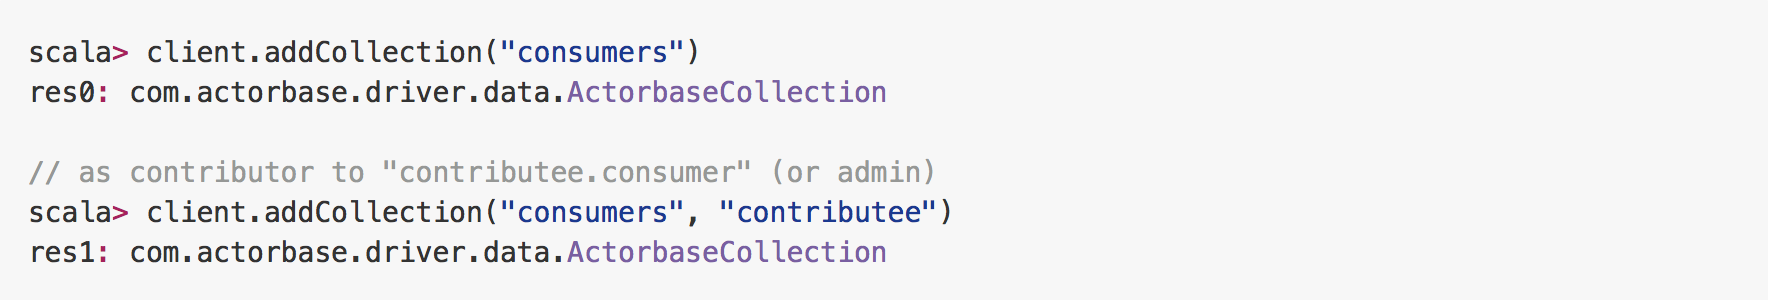
\includegraphics[width=0.9\textwidth,keepaspectratio]{RQ/DevManual/Driver-AddCollection.png}
       \caption{Driver usage: add collection  methods}
     \end{center}
   \end{figure}
  Add collection\textsuperscript{\ref{coll}} method could raise:
  \begin{itemize}
  \item \textbf{CollectionAlreadyExistsExc:} In case the name of the collection\textsuperscript{\ref{coll}} is already taken by another collection\textsuperscript{\ref{coll}} in \textbf{Actorbase};
  \item \textbf{UndefinedCollectionExc:} In case the user tried to insert a new collection\textsuperscript{\ref{coll}} with an empty name.
  \end{itemize}
\item \verb=insert= methods:\\ These methods come in two variants: the first one accepting
  a vararg\footnote{A sequence of arguments} of key-value tuple and the second
  one accepting an
  \verb=ActorbaseObject=\footnote{An object representing a key-value pair inside Actorbase\label{ABobj}} instance;
  e.g.:
   \begin{figure}[H]
     \begin{center}
       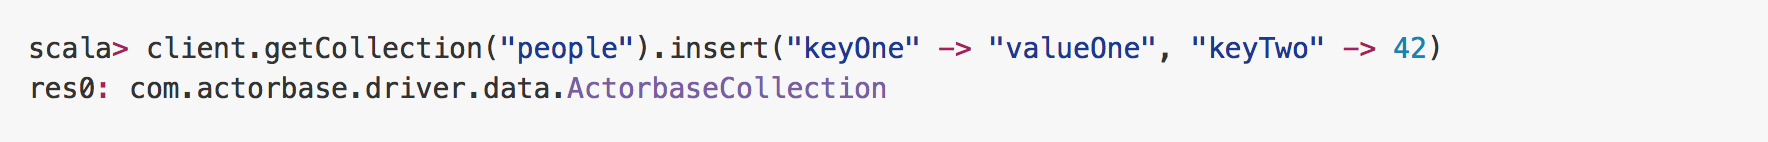
\includegraphics[width=0.9\textwidth,keepaspectratio]{RQ/DevManual/Driver-Insert.png}
       \caption{Driver usage: insertion methods}
     \end{center}
   \end{figure}
  Insert methods could raise:
  \begin{itemize}
  \item \textbf{DuplicateKeyExc:} In case of a key is already taken inside the collection\textsuperscript{\ref{coll}}.
  \end{itemize}
\item \verb=remove= methods:\\ There are two variants of this method too, the usage is
  analogous to insert, e.g.:
   \begin{figure}[H]
     \begin{center}
       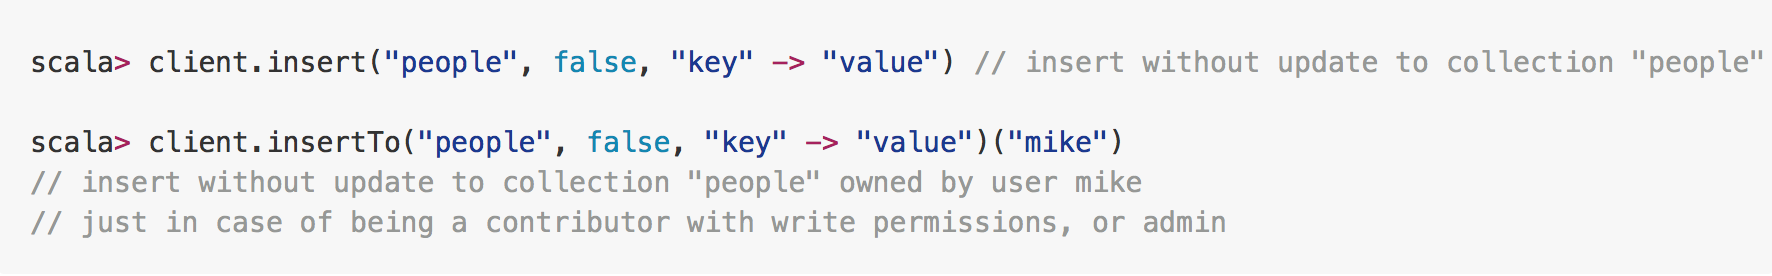
\includegraphics[width=0.9\textwidth,keepaspectratio]{RQ/DevManual/Driver-Insert2.png}
       \caption{Driver usage: remove methods}
     \end{center}
   \end{figure}
\item \verb=find= method:\\ This method accepts one or more \verb=Strings= representing
  keys to be retrieved from the collection\textsuperscript{\ref{coll}}; once again the usage is similar to the insert and
  remove methods, e.g.:
   \begin{figure}[H]
     \begin{center}
       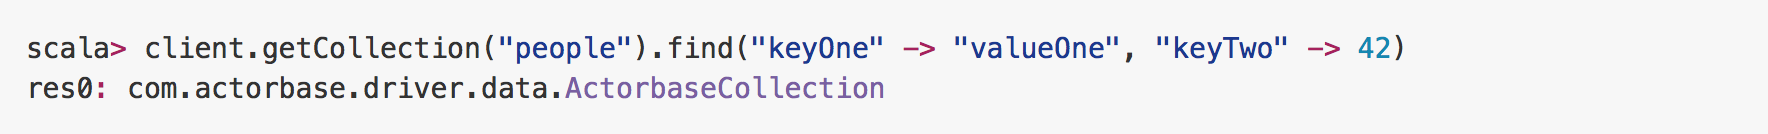
\includegraphics[width=0.9\textwidth,keepaspectratio]{RQ/DevManual/Driver-Find.png}
       \caption{Driver usage: find method}
     \end{center}
   \end{figure}
\item \verb=findOne= method:\\ This method accepts one \verb=ActorbaseObject=\textsuperscript{\ref{ABobj}} representing
  a key-value pair to be retrieved from the collection\textsuperscript{\ref{coll}}; once again the usage is similar to insert and
  remove methods, e.g.:
   \begin{figure}[H]
     \begin{center}
       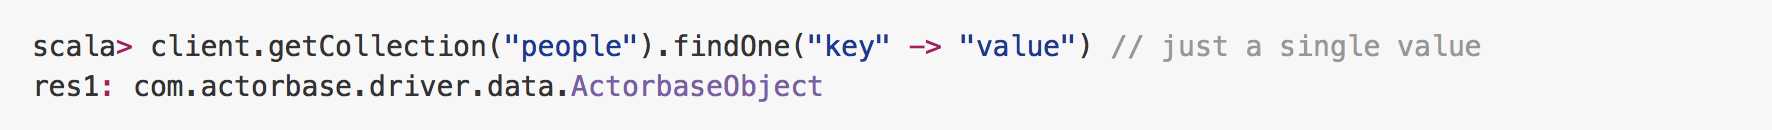
\includegraphics[width=0.9\textwidth,keepaspectratio]{RQ/DevManual/Driver-FindOne.png}
       \caption{Driver usage: findOne method}
     \end{center}
   \end{figure}
\item \verb=drop= methods:\\ Again this method has multiple variants, there is the
  \verb=dropCollections= that can be used to wipe out all the database, e.g.:
   \begin{figure}[H]
     \begin{center}
       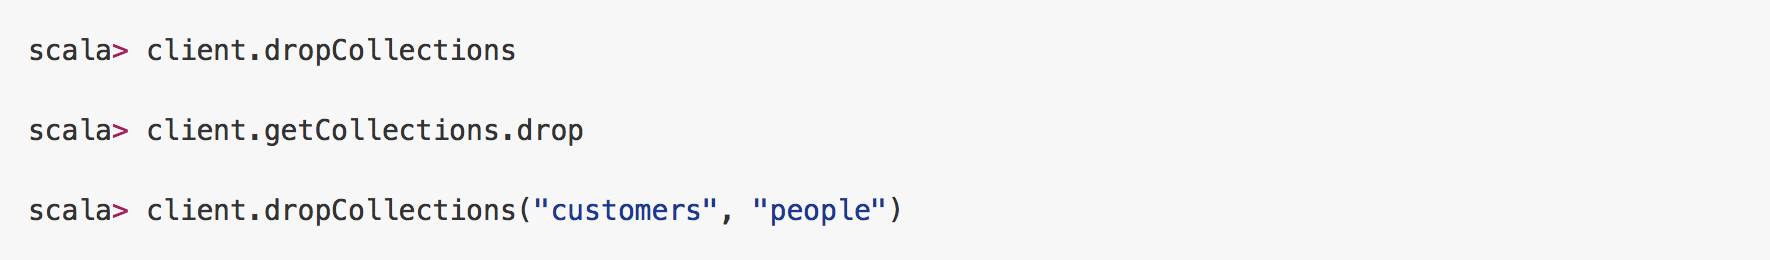
\includegraphics[width=0.9\textwidth,keepaspectratio]{RQ/DevManual/Driver-DropCollections.png}
       \caption{Driver usage: dropCollections method}
     \end{center}
   \end{figure}
  the \verb=drop= inside an \verb=ActorbaseCollection=\textsuperscript{\ref{ABcoll}} object:
   \begin{figure}[H]
     \begin{center}
       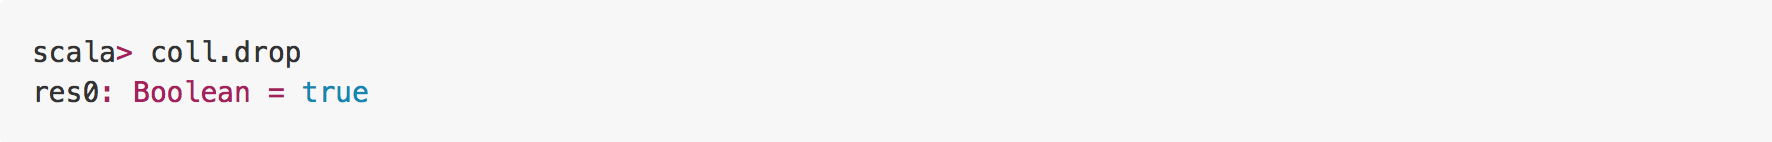
\includegraphics[width=0.9\textwidth,keepaspectratio]{RQ/DevManual/Driver-Drop.png}
       \caption{Driver usage: drop method}
     \end{center}
   \end{figure}
  and finally \verb=drop= inside an \verb=ActorbaseCollectionMap=\textsuperscript{\ref{abcoll}}, it takes a
  vararg of \verb=String= representing a sequence of collections\textsuperscript{\ref{coll}} to be removed
  e.g.:
   \begin{figure}[H]
     \begin{center}
       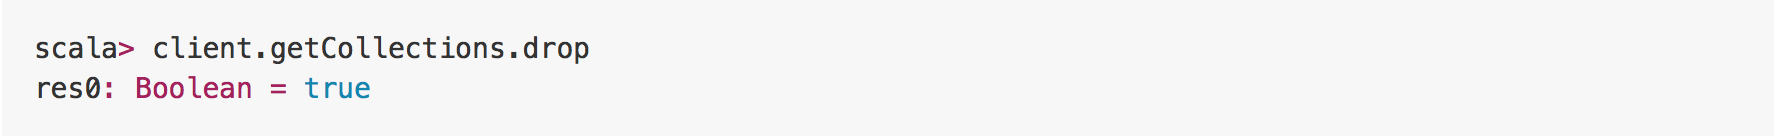
\includegraphics[width=0.9\textwidth,keepaspectratio]{RQ/DevManual/Driver-Drop2.png}
       \caption{Driver usage: drop method}
     \end{center}
   \end{figure}
\item printing collections\textsuperscript{\ref{coll}}:\\All objects returned by \verb=ActorbaseDriver=
  have an override\footnote{Specific implementation of a method in a subclass that
    is already provided by one of its superclasses} to the method \verb=toString=
  that returns a pretty formatted JSON (JavaScript Object Notation) \verb=String=, e.g.:
   \begin{figure}[H]
     \begin{center}
       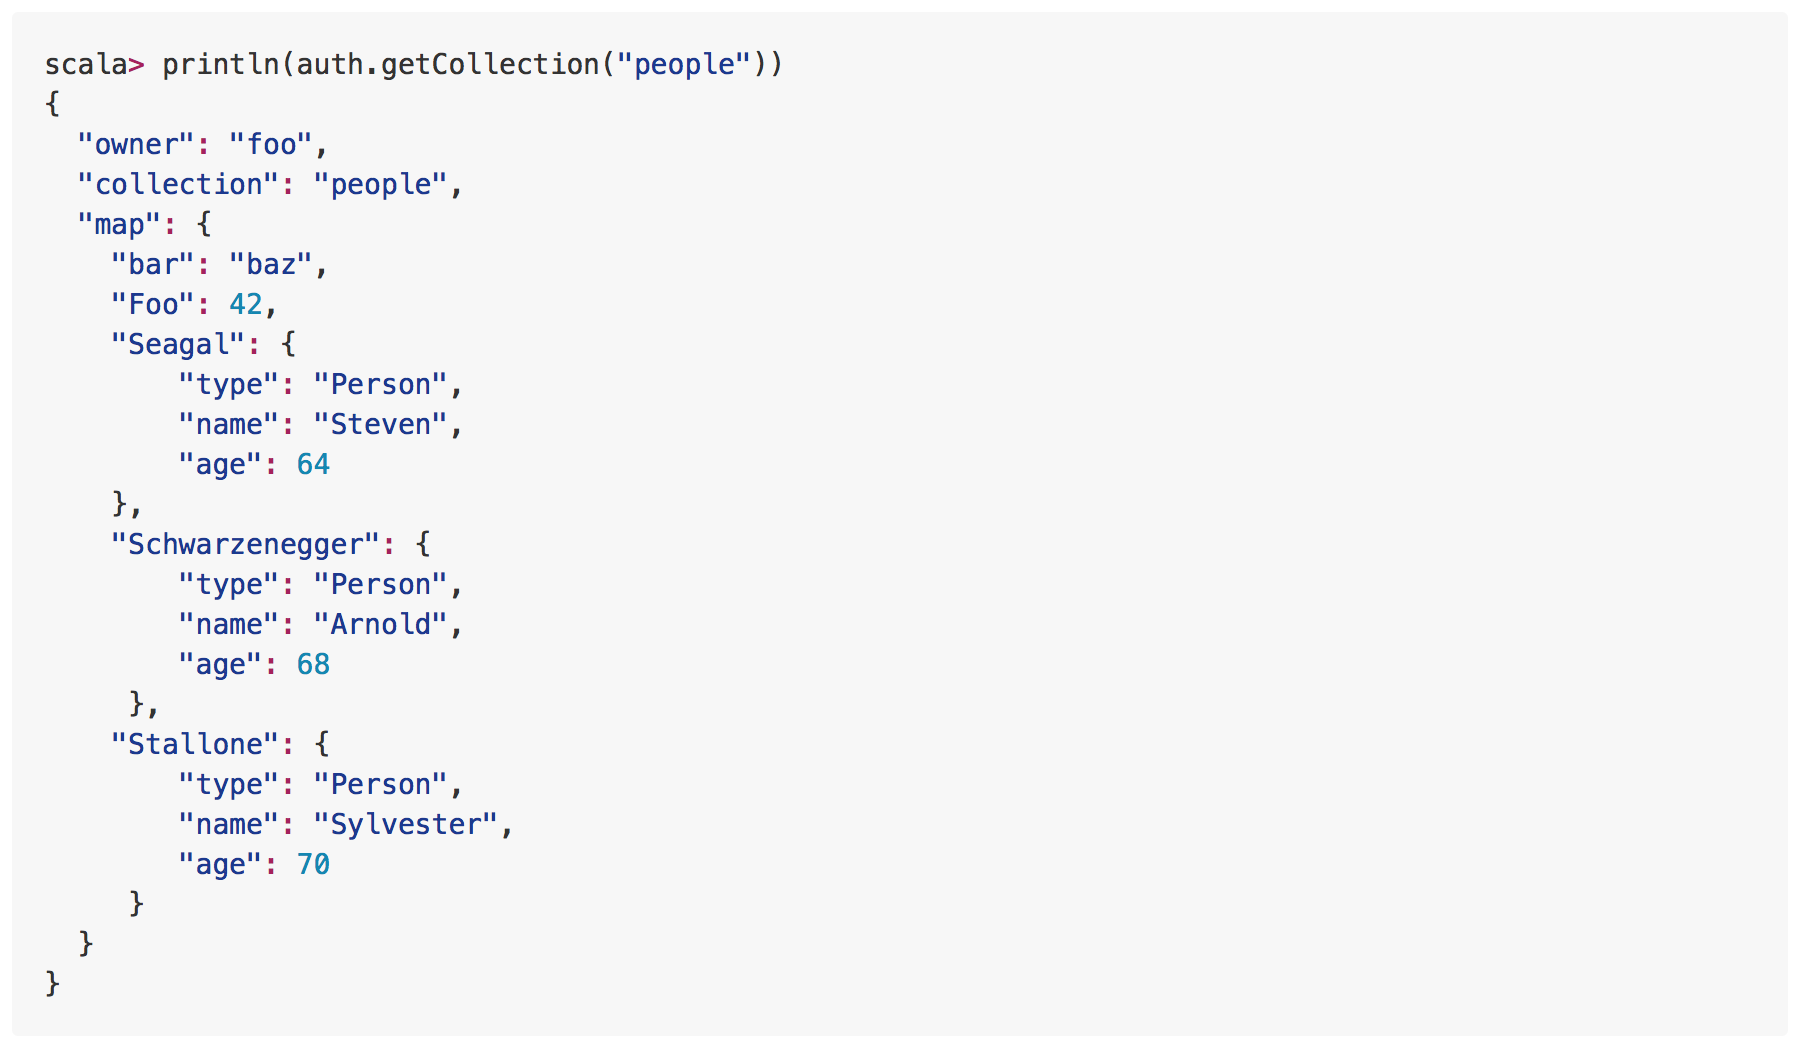
\includegraphics[width=0.9\textwidth,keepaspectratio]{RQ/DevManual/Driver-Printing.png}
       \caption{Driver usage: drop method}
     \end{center}
   \end{figure}
\item \verb=count= elements\footnote{Key-value pairs} inside a collection\textsuperscript{\ref{coll}} e.g.
   \begin{figure}[H]
     \begin{center}
       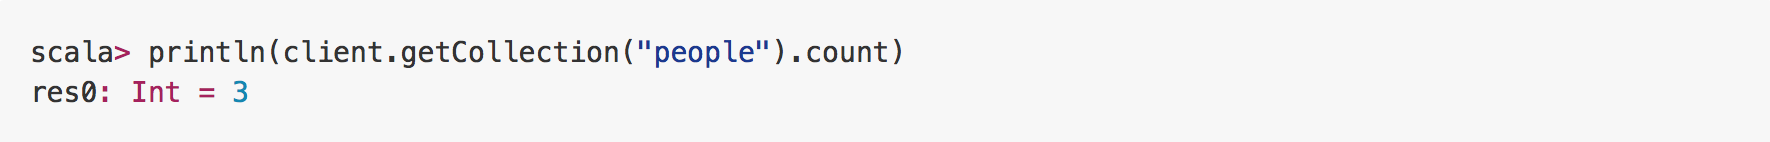
\includegraphics[width=0.9\textwidth,keepaspectratio]{RQ/DevManual/Driver-Counting.png}
       \caption{Driver usage: drop method}
    \end{center}
   \end{figure}
\item \verb=importFromFile=, method that allows to import a (possibly) large number of collections\textsuperscript{\ref{coll}}
  directly into \textbf{Actorbase}
   \begin{figure}[H]
     \begin{center}
       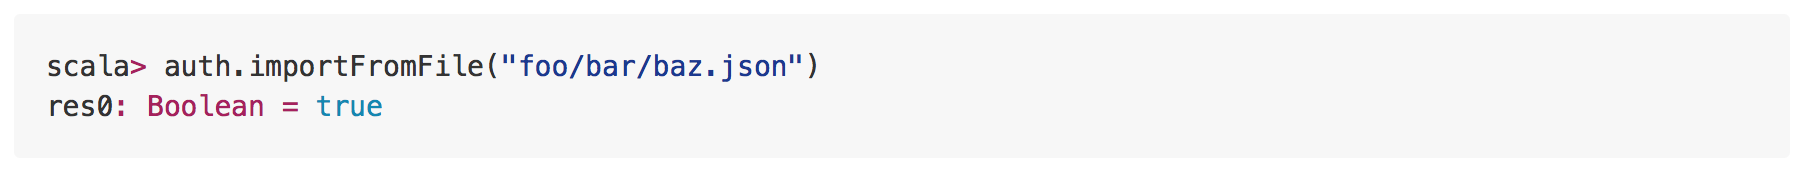
\includegraphics[width=0.9\textwidth,keepaspectratio]{RQ/DevManual/Driver-Import.png}
       \caption{Driver usage: import from file method}
    \end{center}
   \end{figure}
  This method could raise:
  \begin{itemize}
  \item \textbf{UndefinedFileExc:} in case the file has not been found at the given path in the filesystem;
  \item \textbf{MalformedFileExc:} in case the file is not in JSON format or it is not a valid JSON.
  \end{itemize}

\item \verb=exportToFile=, method that allows to export one or more collections\textsuperscript{\ref{col}} to a specified path on the filesystem
   \begin{figure}[H]
     \begin{center}
       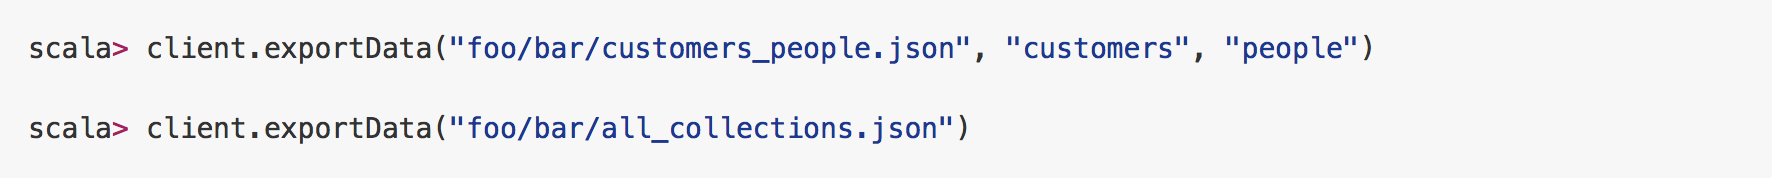
\includegraphics[width=0.9\textwidth,keepaspectratio]{RQ/DevManual/Driver-Export.png}
       \caption{Driver usage: export to file method}
     \end{center}
   \end{figure}
\end{itemize}

\subparagraph{Contributor management}

Each user in \textbf{Actorbase} has the possibility to add and remove contributors
to his collections\textsuperscript{\ref{coll}}, a user can be added with two levels of
permissions:
\begin{itemize}
\item read, means that a user can only make read operations on the collection\textsuperscript{\ref{coll}} without modifying it;
\item read-write, means that a user can make read and write operations on the collection\textsuperscript{\ref{coll}}.
\end{itemize}
e.g.:
 \begin{figure}[H]
   \begin{center}
     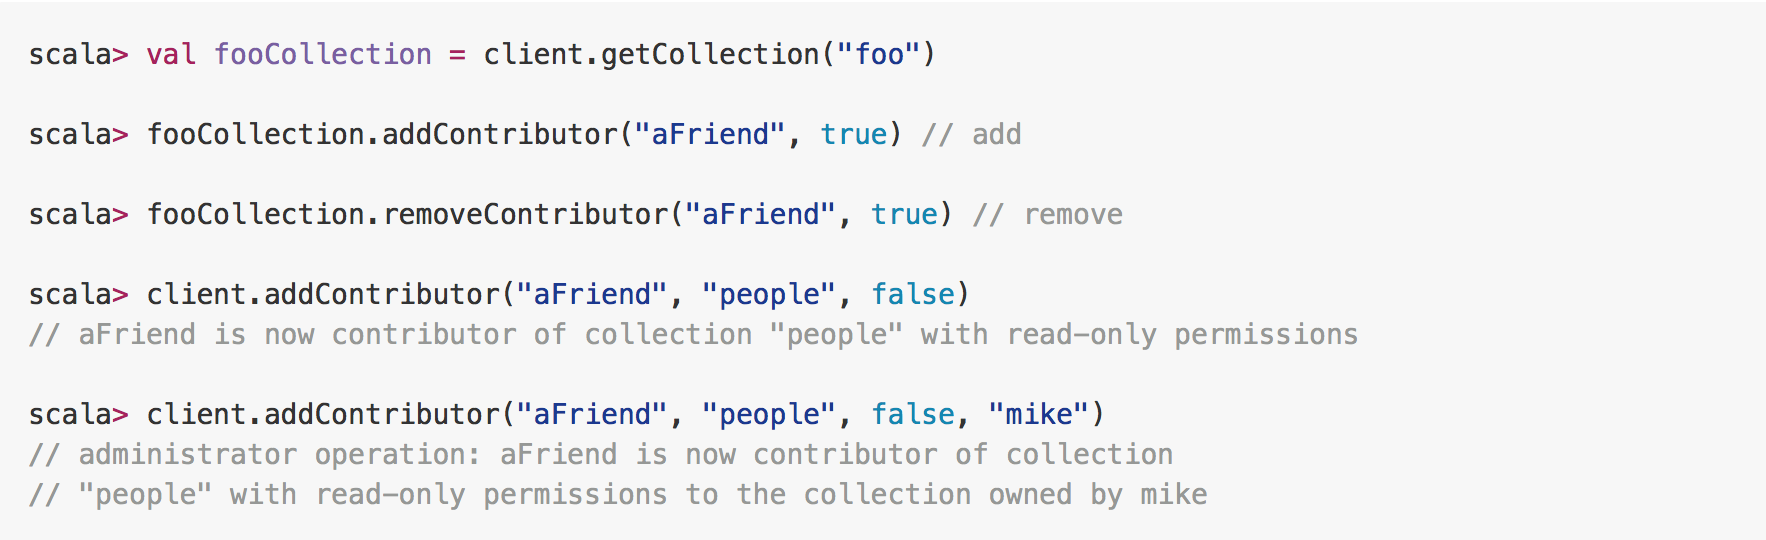
\includegraphics[width=0.9\textwidth,keepaspectratio]{RQ/DevManual/Driver-Contributor.png}
     \caption{Driver usage: drop method}
   \end{center}
 \end{figure}

\subparagraph{Administrative operations}

\textbf{Actorbase} expects two kind of users, common and administrator. The last one has
some privileges over the others, such as a wider range of collections\textsuperscript{\ref{coll}} (all
database) with read-write permissions, and capabilities of adding and removing
users to and from the system, and finally resetting the password of given users.
 \begin{figure}[H]
   \begin{center}
     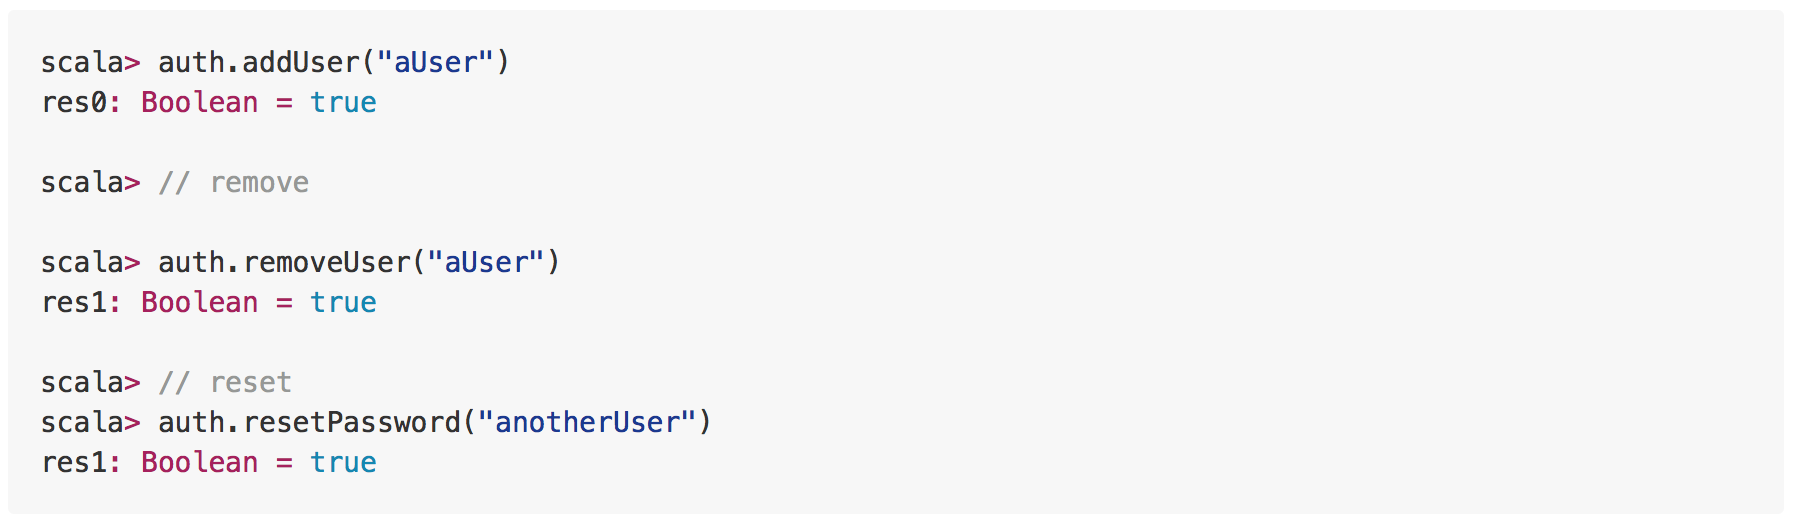
\includegraphics[width=0.9\textwidth,keepaspectratio]{RQ/DevManual/Driver-Administrative.png}
     \caption{Driver usage: drop method}
   \end{center}
 \end{figure}
Administrative operations could raise some exceptions:
\begin{itemize}
\item \textbf{UndefinedUsernameExc:} In case of addition of a new user with an empty username;
\item \textbf{UsernameNotFoundExc:} In case the username inserted in the remove command is not found.
\end{itemize}

\paragraph{Failure management}

In addition to all exceptions that could be raised, there is one error that is
shared by every method and that is in case of a communication error, which can
be caused by not receiving a response from the server in a predetermined time or 
if the destination address is unreachable, the driver will launch a
timeout connection exception.

\paragraph{Contribute}

\subparagraph{Issues}

\textbf{Actorbase} is hosted on github at the url
\url{https://github.com/ScalateKids} divided in two repositories:

\begin{itemize}
\item\textbf{Server-side}
  \begin{itemize}
  \item \textbf{Issue Tracker:} \url{https://github.com/ScalateKids/Actorbase-Server/issues}
  \item \textbf{Source code:} \url{https://github.com/ScalateKids/Actorbase-Server}
  \end{itemize}
\item\textbf{CLI}
  \begin{itemize}
  \item \textbf{Issue Tracker:} \url{https://github.com/ScalateKids/Actorbase-Client/isssues}
  \item \textbf{Source code:} \url{https://github.com/ScalateKids/Actorbase-Client}
  \end{itemize}
\end{itemize}

\subparagraph{Troubleshooting}

If you are having issues or strange malfunctions, please let us know at
\href{mailto:scalatekids@gmail.com}{scalatekids@gmail.com}.

\end{document}